%
% chapter.tex -- Anwendungen von Matrizen in der Codierungstheorie und
%                Kryptographie
%
% (c) 2020 Prof Dr Andreas Müller, Hochschule Rapperswil
%
% !TeX spellcheck = de_CH
\chapter{Anwendungen in Kryptographie und Codierungstheorie
\label{buch:chapter:kryptographie}}
\lhead{Kryptographie und Codierungstheorie}
\rhead{}
Die algebraische Theorie der endlichen Körper hat sich als besonders
nützliche herausgestellt in der Krypographie.
Die Eigenschaften dieser Körper sind reichhaltig genug, um 
kryptographsch widerstandsfähige Algorithmen zu liefern, die
auch in ihrer Stärke beliebig skaliert werden können.
Gleichzeitig liefert die Algebra auch eine effiziente Implementierung.
In diesem Abschnitt soll dies an einigen Beispielen gezeigt werden.

%
% arith.tex
%
% (c) 2021 Prof Dr Andreas Müller, Hochschule Rapperswil
%
\section{Arithmetik für die Kryptographie
\label{buch:section:arithmetik-fuer-kryptographie}}
\rhead{Arithmetik für die Kryptographie}
Die Algorithmen der mathematischen Kryptographie basieren
auf den Rechenoperationen in grossen, aber endlichen Körpern.
Für die Division liefert der euklidische Algorithmus eine
Methode, der in so vielen Schritten die Inverse findet,
wie Dividend und Divisor Binärstellen haben.
Dies ist weitgehend optimal.

Die Division ist umkehrbar, in der Kryptographie strebt man aber an,
Funktionen zu konstruieren, die nur mit grossem Aufwand umkehrbar sind.
Eine solche Funktion ist das Potenzieren in einem endlichen Körper.
Die Berechnung von Potenzen durch wiederholte Multiplikation ist jedoch
prohibitiv aufwendig, daher ist ein schneller Potenzierungsalgorithmus
nötig, der in Abschnitt~\ref{buch:subsection:potenzieren} beschrieben
wird.
Bei der Verschlüsselung grosser Datenmengen wie zum Beispiel bei
der Verschlüsselung ganzer Harddisks mit Hilfe des AES-Algorithmus
kommt es auf die Geschwindigkeit auch der elementarsten Operationen
in den endlichen Körpern an.
Solche Methoden werden in den Abschnitten
\ref{buch:subsection:rechenoperationen-in-fp}
und
\ref{buch:subsection:rechenoperatione-in-f2l}
besprochen.

\subsection{Potenzieren
\label{buch:subsection:potenzieren}}
Wir gehen davon aus, dass wir einen schnellen Algorithmus zur
Berechnung des Produktes zweier Elemente $a,b$ in einer
beliebigen Gruppe $G$ haben.
Die Gruppe $G$ kann die Multiplikation der ganzen oder reellen Zahlen
sein, dies wird zum Beispiel in Implementation der Potenzfunktion
verwendet.
Für kryptographische Anwendungen ist $G$ die multiplikative Gruppe
eines endlichen Körpers oder eine elliptische Kurve.

Zur Berechnung von $a^k$ sind bei einer naiven Durchführung des
Algorithmus $k-1$ Multiplikationen nötig, immer sofort gefolgt
von einer Reduktion $\mod p$ um sicherzustellen, dass die Resultate
nicht zu gross werden.
Ist $l$ die Anzahl der Binärstellen von $k$, dann benötigt dieser
naive Algorithmus $O(2^l)$ Multiplikationen, die Laufzeit wächst
also exponentiell mit der Bitlänge von $k$ an.
Der nachfolgend beschriebene Algorithmus reduziert die Laufzeit auf
die $O(l)$.

Zunächst schreiben wir den Exponenten $k$ in binärer Form als
\[
k = k_l2^l + k_{l-1}2^{l-1} + \dots k_22^2+k_12^1 k_02^0.
\]
Die Potenz $a^k$ kann dann geschrieben werden als
\[
a^k
=
a^{k_l2^l} \cdot a^{k_{l-1}2^{l-1}} \cdot \dots \cdot
a^{k_22^2} \cdot a^{k_12^1} \cdot a^{k_02^0}
\]
Nur diejenigen Faktoren tragen etwas bei, für die $k_i\ne 0$ ist.
Die Potenz kann man daher auch schreiben als
\[
a^k
=
\prod_{k_i\ne 0} a^{2^i}.
\]
Es sind also nur so viele Faktoren zu berücksichtigen, wie $k$ 
Binärstellen $1$ hat.

Die einzelnen Faktoren $a^{2^i}$ können durch wiederholtes Quadrieren
erhalten werden:
\[
a^{2^i} = a^{2\cdot 2^{i-1}} = (a^{2^{i-1}})^2,
\]
also durch maximal $l-1$ Multiplikationen.
Wenn $k$ keine Ganzzahl ist sondern binäre Nachkommastellen hat, also
\[
k=k_l2^l + \dots + k_12^1 + k_02^0 + k_{-1}2^{-1} + k_{-2}2^{-2}+\dots,
\]
dann können die Potenzen $a^{2^{-i}}$ durch wiederholtes Wurzelziehen
\[
a^{2^{-i}} = a^{\frac12\cdot 2^{-i+1}} = \sqrt{a^{2^{-i+1}}}
\]
gefunden werden.
Die Berechnung der Quadratwurzel lässt sich in Hardware effizient
implementieren.

\begin{algorithmus}
Der folgende Algorithmsu berechnet $a^k$ in $O(\log_2(k))$
Multiplikationen
\begin{enumerate}
\item Initialisiere $p=1$ und $q=a$
\item Falls $k$ ungerade ist, setze $p:=p\cdot q$ 
\item Setze $q:=q^2$ und $k := k/2$, wobei die ganzzahlige Division durch $2$
am effizientesten als Rechtsshift implementiert werden kann.
\item Falls $k>0$, fahre weiter bei 2.
\end{enumerate}
\end{algorithmus}

\begin{beispiel}
Die Berechnung von $1.1^{17}$ mit diesem Algorithmus ergibt
\begin{enumerate}
\item $p=1$, $q=1.1$
\item $k$ ist ungerade: $p:=1.1$
\item $q:=q^2=1.21$, $k := 8$
\item $k$ ist gerade
\item $q:=q^2=1.4641$, $k := 4$
\item $k$ ist gerade
\item $q:=q^2=2.14358881$, $k := 2$
\item $k$ ist gerade
\item $q:=q^2=4.5949729863572161$, $k := 1$
\item $k$ ist ungerade: $p:=1.1\cdot p = 5.05447028499293771$
\item $k:=0$
\end{enumerate}
Multiplikationen sind nur nötig in den Schritten 3, 5, 7, 9, 10, es
werden also genau $5$ Multiplikationen ausgeführt.
\end{beispiel}

\subsection{Rechenoperationen in $\mathbb{F}_p$
\label{buch:subsection:rechenoperationen-in-fp}}
Die Multiplikation macht aus zwei Faktoren $a$ und $b$ ein 
Resultat mit Bitlänge $\log_2 a+\log_2 b$, die Bitlänge wird
also typischerweise verdoppelt.
In $\mathbb{F}_p$ muss anschliessend das Resultat $\mod p$
reduziert werden, so dass die Bitlänge wieder höchstens
$\log_2p$ ist.
In folgenden soll gezeigt werden, dass dieser Speicheraufwand 
für eine Binärimplementation deutlich reduziert werden kann,
wenn die Reihenfolge der Operationen modifiziert wird.

Für die Multiplikation von $41\cdot 47$ rechnet man im Binärsystem
\begin{center}
\begin{tabular}{>{$}r<{$}}
\texttt{{\color{darkgreen}1}0{\color{red}1}001}\cdot\texttt{101111}\\
\hline
\texttt{101111}\\
\texttt{{\color{red}101111}\phantom{000}}\\
\texttt{{\color{darkgreen}101111}\phantom{00000}}\\
\hline
\texttt{11110000111}\\
\hline
\end{tabular}
\end{center}
In $\mathbb{F}_{53}$ muss im Anschluss Modulo $p=53$ reduziert werden.

Der Speicheraufwand entsteht zunächst dadurch, dass durch die Multiplikation
mit $2$ die Summanden immer länger werden.
Man kann den die Sumanden kurz halten, indem man jedesmal, wenn 
der Summand nach der Multiplikation mit $2$ grösser als $p$ geworden ist,
$p$ subtrahiert (Abbildung~\ref{buch:crypto:fig:reduktion}).
Ebenso kann bei nach jeder Addition das bereits reduzierten zweiten
Faktors wieder reduziert werden.
Die Anzahl der nötigen Reduktionsoperationen wird durch diese
frühzeitig durchgeführten Reduktionen nicht teurer als bei der Durchführung
des Divisionsalgorithmus.

\begin{figure}
\begin{center}
\begin{tabular}{>{$}r<{$}>{$}r<{$}>{$}r<{$}|>{$}r<{$}>{$}r<{$}>{$}r<{$}}
\text{Multiplikation mit $2$}&\text{Reduktion?}&\text{reduziert}
	&\text{Summanden}&\text{Summe}&\text{reduziert}
\\
\hline
\texttt{101111}               &                &\texttt{101111} 
	&\texttt{101111}&\texttt{101111}&\texttt{101111}
\\
\texttt{101111\phantom{0}}    &\texttt{{\color{red}1011110}}&\texttt{101001}
	&               &               &
\\
\texttt{101111\phantom{00}}   &\texttt{0{\color{red}111010}}&\texttt{011101}
	&               &               &
\\
\texttt{101111\phantom{000}}  &\texttt{0001010}&\texttt{000101}
	&\texttt{000101}&\texttt{110100}&\texttt{110100}
\\
\texttt{101111\phantom{0000}} &\texttt{0010100}&\texttt{001010}
	&               &               &
\\
\texttt{101111\phantom{00000}}&\texttt{0101000}&\texttt{010100}
	&\texttt{010100}&\texttt{{\color{red}1001000}}&\texttt{10011}\rlap{$\mathstrut=19$}
\end{tabular}
\end{center}
\caption{Multiplikation von $41=\texttt{101001}_2$ mit $47=\texttt{101111}_2$,
Reduktion nach jeder Multiplikation mit $2$: falls das Resultat
$>p$ ist, wie in den rot markierten Zeilen $p=53=\texttt{110101}_2$
durchgeführt.
Bei der Bildung der Summe wird ebenfalls in jedem Schritt falls nötig
reduziert, angezeigt durch die roten Zahlen in der zweitletzten
Spalte.
Die Anzahl der Subtraktionen, die für die Reduktionen nötig sind, ist
von der selben Grössenordnung wie bei der Durchführung des
Divisionsalgorithmus.
\label{buch:crypto:fig:reduktion}}
\end{figure}

Es ist also möglich, mit gleichem Aufwand an Operationen
aber mit halbe Speicherplatzbedarf die Multiplikationen in $\mathbb{F}_p$
durchzuführen.
Die Platzeinsparung ist besonders bei Implementationen in Hardware 
hilfreich, wo on-die Speicherplatz teuer sein kann.

\subsection{Rechenoperationen in $\mathbb{F}_{2^l}$
\label{buch:subsection:rechenoperatione-in-f2l}}
Von besonderem praktischem Interesse sind die endlichen Körper
$\mathbb{F}_{2^l}$.
Die arithmetischen Operationen in diesen Körpern lassen sich besonders
effizient in Hardware realisieren.

\subsubsection{Zahldarstellung}
Ein endlicher Körper $\mathbb{F}_{2^l}$ ist definiert durch ein
irreduzibles Polynom in $\mathbb{F}_2[X]$ vom Grad $2^l$ 
\[
m(X)
=
X^l + m_{l-1}X^{l-1} + m_{l-2}X^{l-2} + \dots + m_2X^2 + m_1X + m_0
\]
gegeben.
Ein Element in $\mathbb{F}_2[X]/(m)$ kann dargestellt werden durch ein
Polynom vom Grad $l-1$, also durch
\[
a = a_{l-1}X^{l-1} + a_{l-2}X^{l-2} +\dots + a_2X^2 + a_1X + a_0.
\]
In einer Maschine kann eine Zahl also als eine Bitfolge der Länge $l$
dargestellt werden.

\subsubsection{Addition}
Die Addition in $\mathbb{F}_2$ ist in Hardware besonders leicht zu
realisieren.
Die Addition ist die XOR-Operation, die Multiplikation ist die UND-Verknüfung.
Ausserdem stimmen in $\mathbb{F}_2$ Addition und Subtraktion überein.

Die Addition zweier Polynome erfolgt komponentenweise.
Die Addition von zwei Elemente von $\mathbb{F}_{2^l}$ kann also
durch die bitweise XOR-Verknüpfung der Darstellungen der Summanden 
erfolgen.
Diese Operation ist in einem einzigen Maschinenzyklus realisierbar.
Die Subtraktion, die für die Reduktionsoperation module $m(X)$ nötig
ist, ist mit der Addition identisch.

\subsubsection{Multiplikation}
Die Multiplikation zweier Polynome benötigt zunächst die Multiplikation
mit $X$, wodurch der Grad des Polynoms ansteigt und möglicherweise so
gross wird, dass eine Reduktionsoperation modulo $m(X)$ nötig wird.
Die Reduktion wird immer dann nötig, wenn der Koeffizient von $X^l$
nicht $0$ ist.
Der Koeffizient kann dann zum Verschwinden gebracht werden, indem
$m(X)$ addiert wird.

\begin{figure}
\centering
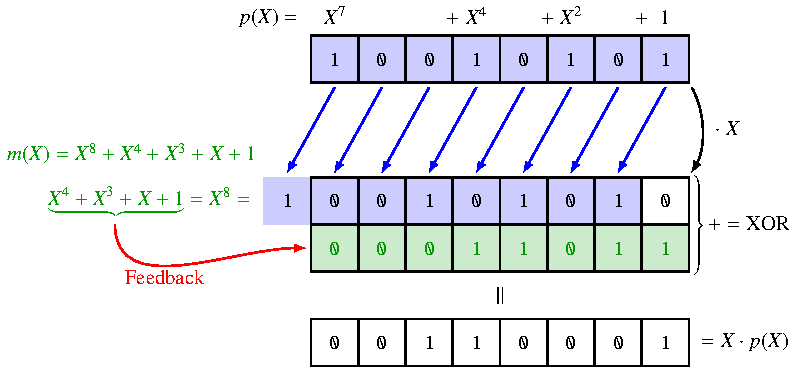
\includegraphics{chapters/90-crypto/images/schieberegister.pdf}
\caption{Implementation der Multiplikation mit $X$ in einem 
endlichen Körper $\mathbb{F}_{2^l}$ mit dem Minimalpolynom
$m(X) = X^8+X^4+X^3+X^+1$ als Feedback-Schieberegister.
\label{buch:crypto:fig:schieberegister}}
\end{figure}

In Abbildung~\ref{buch:crypto:fig:schieberegister} wird gezeigt,
wie die Reduktion erfolgt, wenn die Multiplikation mit $X$, also der
Shift nach links, einen Überlauf ergibt.
Das Minimalpolynom $m(X)=X^8+X^4+X^3+X+1$ bedeutet, dass in $\mathbb{F}_{2^l}$
$X^8=X^4+X^3+X+1$ gilt, so dass man das Überlaufbit durch 
$X^4+X^3+X+1$ ersetzen und addieren kann.

Ein Produktes $p(X)\cdot q(X)$, wobei $p(X)$ und
$q(X)$ Repräsentaten von Elementen $\mathbb{F}_{2^l}$ sind, kann jetzt
wie folgt berechnet werden.
Mit dem Schieberegister werden die Vielfachen $X^k\cdot p(X)$ 
für $k=0,\dots,l-1$ berechnet.
Diejenigen Vielfachen, für die der Koeffizient von $X^k$ in $q(X)$
von $0$ verschieden ist werden aufsummiert und ergeben das Produkt.
Der Prozess in Abbildung~\ref{buch:crypto:fig:multiplikation}
dargestellt.

\begin{figure}
\centering
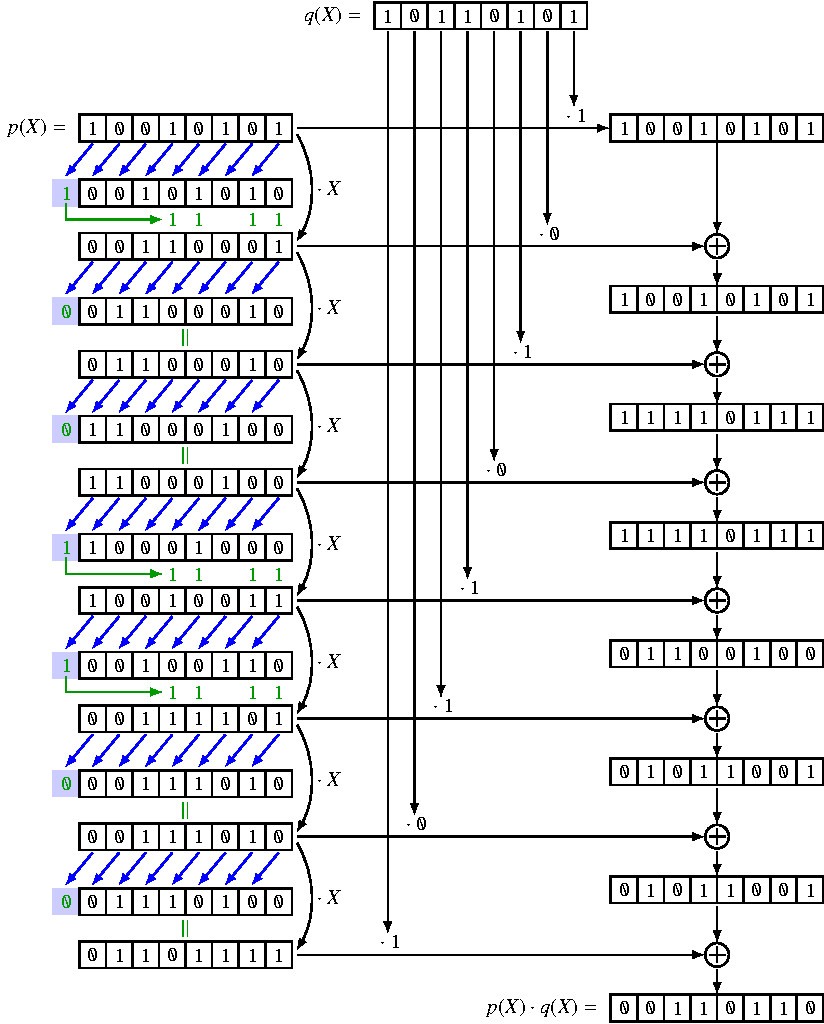
\includegraphics[width=\textwidth]{chapters/90-crypto/images/multiplikation.pdf}
\caption{Multiplikation zweier Elemente von $\mathbb{F}_{2^l}$.
Mit Hilfe des Schieberegisters am linken Rand werden die Produkte 
$X\cdot p(X)$, $X^2\cdot p(X),\dots,X^7\cdot p(X)$ nach der in
Abbildung~\ref{buch:crypto:fig:schieberegister} dargestellten
Methode berechnet.
Am rechten Rand werden diejenigen $X^k\cdot p(X)$ aufaddiert,
für die der $X^k$-Koeffizient von $q(X)$ von $0$ verschieden ist.
\label{buch:crypto:fig:multiplikation}}
\end{figure}


% XXX Beispiel F einer Oakley-Gruppe


%
% ff.tex -- Kryptographie und endliche Körper
%
% (c) 2020 Prof Dr Andreas Müller, Hochschule Rapperswil
%

\section{Kryptographie und endliche Körper
\label{buch:section:kryptographie-und-endliche-koerper}}
\rhead{Kryptographie und endliche Körper}

\subsection{Potenzen in $\mathbb{F}_p$ und diskreter Logarithmus
\label{buch:subsection:potenzen-diskreter-logarithmus}}
Für kryptographische Anwendungen wird eine einfach zu berechnende
Funktion benötigt,
die ohne zusätzliches Wissen, üblicherweise der Schlüssel genannt,
nicht ohne weiteres umkehrbar ist.
Die arithmetischen Operationen in einem endlichen Körper sind
mit geringem Aufwand durchführbar.
Für die ``schwierigste'' Operation, die Division, steht der
euklidische Algorithmus zur Verfügung.

Die nächstschwierigere Operation ist die Potenzfunktion.
Für $g\in \Bbbk$ und $a\in\mathbb{N}$ ist die Potenz $g^a\in\Bbbk$
natürlich durch die wiederholte Multiplikation definiert.
In der Praxis werden aber $g$ und $a$ Zahlen mit vielen Binärstellen
sein, die die wiederholte Multiplikation ist daher sicher nicht
effizient, das Kriterium der einfachen Berechenbarkeit scheint
also nicht erfüllt.
Der folgende Algorithmus berechnet die Potenz in $O(\log_2 a$
Multiplikationen.

\begin{algorithmus}[Divide-and-conquer]
\label{buch:crypto:algo:divide-and-conquer}
Sei $a=a_0 + a_12^1 + a_22^2 + \dots + a_k2^k$ die Binärdarstellung
der Zahl $a$.
\begin{enumerate}
\item setze $f=g$, $x=1$, $i=0$
\label{divide-and-conquer-1}
\item solange $i\ge k$ ist, führe aus
\label{divide-and-conquer-2}
\begin{enumerate}
\item
\label{divide-and-conquer-3}
falls $a_i=1$ setze $x \coloneqq x \cdot f$
\item
\label{divide-and-conquer-4}
$i \coloneqq i+1$ und $f\coloneqq f\cdot f$
\end{enumerate}
\end{enumerate}
Die Potenz $x=g^a$ kann so in $O(\log_2a)$ Multiplikationen
berechnet werden.
\end{algorithmus}

\begin{proof}[Beweis]
Die Initalisierung in Schritt~\ref{divide-and-conquer-1} stellt sicher,
dass $x$ den Wert $g^0$ hat. 
Schritt~\ref{divide-and-conquer-4} stellt sicher,
dass die Variable $f$ immer den Wert $g^{2^i}$ hat.
Im Schritt~\ref{divide-and-conquer-3} wird zu $x$ die Potenz
$g^{a_i2^i}$ hinzumultipliziert.
Am Ende des Algorithmus hat daher $x$ den Wert
\[
x = g^{a_02^0} \cdot g^{a_12^1} \cdot g^{a_22^2} \cdot\ldots\cdot 2^{a_k2^k}
=
g^{a_0+a_12+a_22^2+\dots+a_k2^k}
=
g^a.
\]
Die Schleife wird $\lfloor1+\log_2ab\rfloor$ mal durchlaufen.
In jedem Fall wird auf jeden Fall die Multiplikation in 
Schritt~\ref{divide-and-conquer-4} durchgeführt
und im schlimmsten Fall auch noch die Multiplikation in
Schritt~\ref{divide-and-conquer-3}.
Es werden also nicht mehr als $2\lfloor 1+\log_2a\rfloor=O(\log_2a)$
Multiplikationen durchgeführt.
\end{proof}

\begin{beispiel}
Man berechne die Potenz $7^{2021}$ in $\mathbb{F}_p$.
Die Binärdarstellung von 2021 ist $2021_{10}=\texttt{11111100101}_2$.
Wir stellen die nötigen Operationen des
Algorithmus~\ref{buch:crypto:algo:divide-and-conquer} in der folgenden
Tabelle
\begin{center}
\begin{tabular}{|>{$}r<{$}|>{$}r<{$}|>{$}r<{$}|>{$}r<{$}|}
\hline
 i&   f& a_i&    x\\
\hline
 0&   7&   1&    7\\
 1&  49&   0&    7\\
 2&1110&   1&   24\\
 3& 486&   0&   24\\
 4&1234&   0&   24\\
 5& 667&   1&  516\\
 6& 785&   1&  977\\
 7& 418&   1&  430\\
 8& 439&   1&  284\\
 9& 362&   1&  819\\
10& 653&   1&  333\\
\hline
\end{tabular}
\end{center}
Daraus liest man ab, dass $7^{2021}=333\in\mathbb{F}_{1291}$.
\end{beispiel}

Die Tabelle suggeriert, dass die Potenzen von $g$ ``wild'', also
scheinbar ohne System in $\mathbb{F}_p$ herumspringen.
Dies deutet an, dass die Umkehrung der Exponentialfunktion in $\mathbb{F}_p$
schwierig ist.
Die Umkehrfunktion der Exponentialfunktion, die Umkehrfunktion von 
$x\mapsto g^x$ in $\mathbb{F}_p$ heisst der {\em diskrete Logarithmus}.
\index{diskreter Logarithmus}%
Tatsächlich ist der diskrete Logarithmus ähnlich schwierig zu bestimmen
wie das Faktorisieren von Zahlen, die das Produkt grosser
Primafaktoren ähnlicher Grössenordnung wie $p$ sind.
Die Funktion $x\mapsto g^x$ ist die gesuchte, schwierig zu invertierende
Funktion.

Auf dern ersten Blick scheint der
Algorithmus~\ref{buch:crypto:algo:divide-and-conquer}
den Nachteil zu haben, dass erst die Binärdarstellung der Zahl $a$ 
ermittelt werden muss.
In einem Computer ist dies aber normalerweise kein Problem, da $a$
im Computer ohnehin binär dargestellt ist.
Die Binärziffern werden in der Reihenfolge vom niederwertigsten zum
höchstwertigen Bit benötigt.
Die folgende Modifikation des Algorithmus ermittelt laufend
auch die Binärstellen von $a$.
Die dazu notwendigen Operationen sind im Binärsystem besonders
effizient implementierbar, die Division durch 2 ist ein Bitshift, der
Rest ist einfach das niederwertigste Bit der Zahl.

\begin{algorithmus}
\label{buch:crypto:algo:divide-and-conquer2}
\begin{enumerate}
\item
Setze $f=g$, $x=1$, $i=0$
\item
Solange $a>0$ ist, führe aus
\begin{enumerate}
\item
Verwende den euklidischen Algorithmus um $r$ und $b$ zu bestimmen mit $a=2b+r$
\item
Falls $r=1$ setze $x \coloneqq x \cdot f$
\item
$i \coloneqq i+1$, $a = b$ und $f\coloneqq f\cdot f$
\end{enumerate}
\end{enumerate}
Die Potenz $x=g^a$ kann so in $O(\log_2a)$ Multiplikationen
berechnet werden.
\end{algorithmus}


%
% Diffie-Hellman Schlüsseltausch
%
\subsection{Diffie-Hellman-Schlüsseltausch
\label{buch:subsection:diffie-hellman}}
Eine Grundaufgabe der Verschlüsselung im Internet ist, dass zwei
Kommunikationspartner einen gemeinsamen Schlüssel für die Verschlüsselung
der Daten aushandeln können müssen.
Es muss davon ausgegangen werden, dass die Kommunikation abgehört wird.
Trotzdem soll es für einen Lauscher nicht möglich sein, den 
ausgehandelten Schlüssel zu ermitteln.

% XXX Historisches zu Diffie und Hellman

Die beiden Partner $A$ und $B$ einigen sich zunächst auf eine Zahl $g$,
die öffentlich bekannt sein darf.
Weiter erzeugen sie eine zufällige Zahl $a$ und $b$, die sie geheim
halten.
Das Verfahren soll aus diesen beiden Zahlen einen Schlüssel erzeugen,
den beide Partner berechnen können, ohne dass sie $a$ oder $b$ 
übermitteln müssen.
Die beiden Zahlen werden daher auch die privaten Schlüssel genannt.

Die Idee von Diffie und Hellman ist jetzt, die Werte $x=g^a$ und $y=g^b$
zu übertragen.
In $\mathbb{R}$ würden dadurch natürlich dem Lauscher auch $a$ offenbart,
er könnte einfach $a=\log_g x$ berechnen.
Ebenso kann auch $b$ als $b=\log_g y$ erhalten werden, die beiden
privaten Schlüssel wären also nicht mehr privat.
Statt der Potenzfunktion in $\mathbb{R}$ muss also eine Funktion
verwendet werden, die nicht so leicht umgekehrt werden kann.
Die Potenzfunktion in $\mathbb{F}_p$ erfüllt genau diese Eigenschaft.
Die Kommunikationspartner einigen sich also auch noch auf die (grosse)
Primzahl $p$ und übermitteln $x=g^a\in\mathbb{F}_p$ und
$y=g^b\in\mathbb{F}_p$.

\begin{figure}
\centering
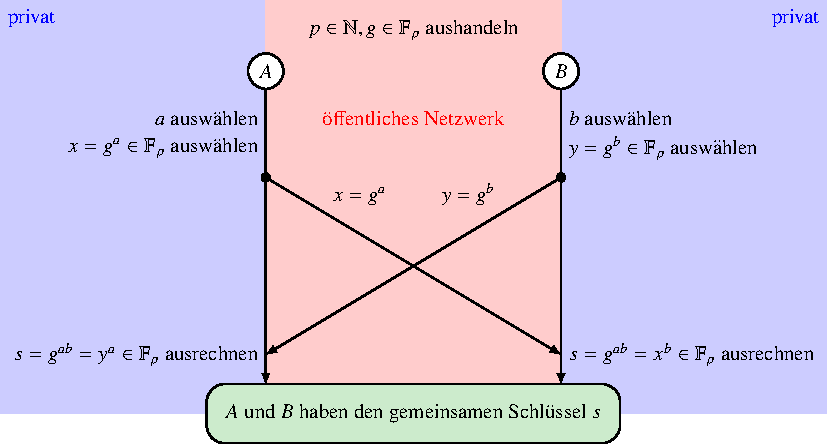
\includegraphics{chapters/90-crypto/images/dh.pdf}
\caption{Schlüsselaustausch nach Diffie-Hellman.
Die Kommunikationspartner $A$ und $B$ einigen sich öffentlich auf
$p\in\mathbb{N}$ und $g\in\mathbb{F}_p$.
$A$ wählt dann einen privaten Schlüssel $a\in\mathbb{N}$ und
$B$ wählt $b\in\mathbb{N}$, sie tauschen dann $x=g^a$ und $y=g^b$
aus.
$A$ erhält den gemeinsamen Schlüssel aus $y^a$, $B$ erhält ihn
aus $x^b$.
\label{buch:crypto:fig:dh}}
\end{figure}

Aus $x$ und $y$ muss jetzt der gemeinsame Schlüssel abgeleitet werden.
$A$ kennt $y=g^b$ und $a$, $B$ kennt $x=g^a$ und $b$.
Beide können die Zahl $s=g^{ab}\in\mathbb{F}_p$ berechnen.
$A$ macht das, indem er $y^a=(g^b)^a = g^{ab}$ rechnet,
$B$ rechnet $x^b = (g^a)^b = g^{ab}$, beide natürlich in $\mathbb{F}_p$.
Der Lauscher kann aber $g^{ab}$ nicht ermitteln, dazu müsste er
$a$ oder $b$ ermitteln können.
Die Zahl $s=g^{ab}$ kann also als gemeinsamer Schlüssel verwendet
werden.



\subsection{Elliptische Kurven
\label{buch:subsection:elliptische-kurven}}
Das Diffie-Hellman-Verfahren basiert auf der Schwierigkeit, in einem 
Körper $\mathbb{F}_p$ die Gleichung $a^x=b$ nach $x$ aufzulösen.
Die Addition in $\mathbb{F}_p$ wird dazu nicht benötigt.
Es reicht, eine Menge mit einer Multiplikation zu haben, in der das
die Gleichung $a^x=b$ schwierig zu lösen ist.
Ein Gruppe wäre also durchaus ausreichend.

Ein Kandidat für eine solche Gruppe könnte der Einheitskreis
$S^1=\{z\in\mathbb{C}\;|\; |z|=1\}$ in der komplexen Ebene sein.
Wählt man eine Zahl $g=e^{i\alpha}$, wobei $\alpha$ ein irrationales
Vielfaches von $\pi$ ist, dann sind alle Potenzen $g^n$ für natürliche
Exponenten voneinander verschieden.
Wäre nämlich $g^{n_1}=g^{n_2}$, dann wäre $e^{i\alpha(n_1-n_2)}=1$ und
somit müsste $\alpha=2k\pi/(n_1-n_2)$ sein.
Damit wäre aber $\alpha$ ein rationales Vielfaches von $\pi$, im Widerspruch
zur Voraussetzung.
Die Abbildung $n\mapsto g^n\in S^1$ ist auf den ersten Blick etwa ähnlich
undurchschaubar wie die Abbildung $n\mapsto g^n\in\mathbb{F}_p$.
Es gibt zwar die komplexe Logarithmusfunktion, mit der man $n$ bestimmen
kann, dazu muss man aber den Wert von $g^n$ mit beliebiger Genauigkeit
kennen, denn die Werte von $g^n$ können beliebig nahe beieinander liegen.

Der Einheitskreis ist die Lösungsmenge der Gleichung $x^2+y^2=1$ für
reelle Koordinaten $x$ und $y$,
doch Rundungsunsicherheiten verunmöglichen den Einsatz in einem 
Verfahren ähnlich dem Diffie-Hellman-Verfahren.
Dieses Problem kann gelöst werden, indem für die Variablen Werte
aus einem endlichen Körper verwendet werden.
Gesucht ist also eine Gleichung in zwei Variablen, deren Lösungsmenge
in einem endlichen Körper eine Gruppenstruktur trägt.
Die Lösungsmenge ist eine ``Kurve'' von Punkten mit
Koordinaten in einem endlichen Körper.

In diesem Abschnitt wird gezeigt, dass sogenannte elliptische Kurven
über endlichen Körpern genau die verlangen Eigenschaften haben.

\subsubsection{Elliptische Kurven}
Elliptische Kurven sind Lösungen einer Gleichung der Form
\begin{equation}
Y^2+XY=X^3+aX+b
\label{buch:crypto:eqn:ellipticcurve}
\end{equation}
mit Werten von $X$ und $Y$ in einem geeigneten Körper.
Die Koeffizienten $a$ und $b$ müssen so gewählt werden, dass die
Gleichung~\eqref{buch:crypto:eqn:ellipticcurve} genügend viele
Lösungen hat.
Über den komplexen Zahlen hat die Gleichung natürlich für jede Wahl von
$X$ drei Lösungen.
Für einen endlichen Körper können wir dies im allgemeinen nicht erwarten,
aber wenn wir genügend viele Wurzeln zu $\mathbb{F}$ hinzufügen können wir
mindestens erreichen, dass die Lösungsmenge so viele Elemente hat, 
dass ein Versuch, die Gleichung $g^x=b$ mittels Durchprobierens zu
lösen, zum Scheitern verurteil ist.

\begin{definition}
\label{buch:crypto:def:ellipticcurve}
Die {\em elliptische Kurve} $E_{a,b}(\Bbbk)$ über dem Körper $\Bbbk$ ist 
die Menge
\[
E_{a,b}(\Bbbk)
=
\{(X,Y)\in\Bbbk^2\;|\;Y^2+XY=X^3+aX+b\},
\]
für $a,b\in\Bbbk$.
\end{definition}

Um die Anschauung zu vereinfachen, werden wir elliptische Kurven über
dem Körper $\mathbb{R}$ visualisieren.
Die daraus gewonnenen geometrischen Einsichten werden wir anschliessend
algebraisch umsetzen.
In den reellen Zahlen kann man die
Gleichung~\eqref{buch:crypto:eqn:ellipticcurve}
noch etwas vereinfachen.
Indem man in \eqref{buch:crypto:eqn:ellipticcurve} 
quadratisch ergänzt, bekommt man
\begin{align}
Y^2 + XY + \frac14X^2 &= X^3+\frac14 X^2 +aX+b
\notag
\\
\Rightarrow\qquad
v^2&=X^3+\frac14X^2+aX+b,
\label{buch:crypto:eqn:ell2}
\end{align}
indem man $v=Y+\frac12X$ setzt.
Man beachte, dass man diese Substition nur machen kann, wenn $\frac12$
definiert ist.
In $\mathbb{R}$ ist dies kein Problem, aber genau über den Körpern
mit Charakteristik $2$, die wir für die Computer-Implementation
bevorzugen, ist dies nicht möglich.
Es geht hier aber nur um die Visualisierung.

Auch die Form \eqref{buch:crypto:eqn:ell2} lässt sich noch etwas 
vereinfachen.
Setzt man $X=u-\frac1{12}$, dann verschwindet nach einiger Rechnung,
die wir hier nicht durchführen wollen, der quadratische Term
auf der rechten Seite.
Die interessierenden Punkte sind Lösungen der einfacheren Gleichung
\begin{equation}
v^2
=
u^3+\biggl(a-\frac{1}{48}\biggr)u + b-\frac{a}{12}+\frac{1}{864}
=
u^3+Au+B.
\label{buch:crypto:ellvereinfacht}
\end{equation}
In dieser Form ist mit $(u,v)$ immer auch $(u,-v)$ eine Lösung,
die Kurve ist symmetrisch bezüglich der $u$-Achse.
Ebenso kann man ablesen, dass nur diejenigen $u$-Werte möglich sind,
für die das kubische Polynom $u^3+Au+B$ auf der rechten Seite von
\eqref{buch:crypto:ellvereinfacht}
nicht negativ ist.

Sind $u_1$, $u_2$ und $u_3$ die Nullstellen des kubischen Polynoms
auf der rechten Seite von~\eqref{buch:crypto:ellvereinfacht}, folgt
\[
v^2
=
(u-u_1)(u-u_2)(u-u_3)
=
u^3
-(u_1+u_2+u_3)u^2
+(u_1u_2+u_1u_3+u_2u_3)u
-
u_1u_2u_3.
\]
Durch Koeffizientenvergleich sieht man, dass $u_1+u_2+u_3=0$ sein muss.
\begin{figure}
\centering
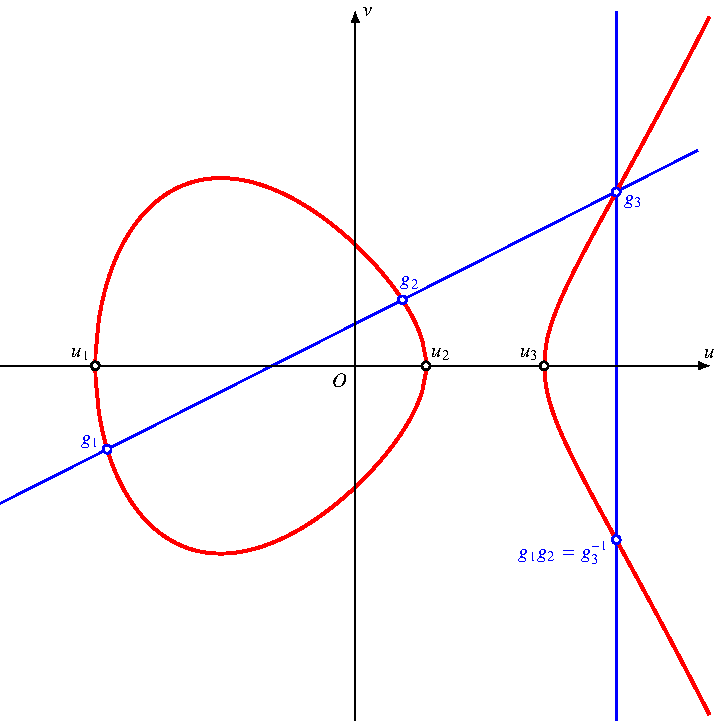
\includegraphics{chapters/90-crypto/images/elliptic.pdf}
\caption{Elliptische Kurve in $\mathbb{R}$ in der Form
$v^2=u^3+Au+B$ mit Nullstellen $u_1$, $u_2$ und $u_3$ des
kubischen Polynoms auf der rechten Seite.
Die blauen Punkte und Geraden illustrieren die Definition der
Gruppenoperation in der elliptischen Kurve.
\label{buch:crypto:fig:elliptischekurve}}
\end{figure}
Abbildung~\ref{buch:crypto:fig:elliptischekurve}
zeigt eine elliptische Kurve in der Ebene.

\subsubsection{Gruppenoperation}

\subsubsection{Beispiele}


%
% aes.tex -- Beschreibung des AES Algorithmus
%
% (c) 2020 Prof Dr Andreas Müller, Hochschule Rapperswil
%
\section{Advanced Encryption Standard -- AES
\label{buch:section:aes}}
\rhead{Advanced Encryption Standard}
Eine wichtige Forderung bei der Konzeption des damals neuen
Advanced Encryption Standard war, dass darin keine ``willkürlich''
erscheinenden Operationen geben darf, bei denen der Verdacht
entstehen könnte, dass sich dahinter noch offengelegtes Wissen
über einen möglichen Angriff auf den Verschlüsselungsalgorithmus
verbergen könnte.
Dies war eine Schwäche des vor AES üblichen DES Verschlüsselungsalgorithmus.
In seiner Definition kommt eine Reihe von Konstanten vor, über deren
Herkunft nichts bekannt war.
Die Gerüchteküche wollte wissen, dass die NSA die Konstanten aus dem
ursprünglichen Vorschlag abgeändert habe, und dass dies geschehen sei,
um den Algorithmus durch die NSA angreifbar zu machen.

Eine weiter Forderung war, dass die Sicherheit des neuen
Verschlüsselungsstandards ``skalierbar'' sein soll, dass man also
die Schlüssellänge mit der Zeit von 128~Bit auf 196 oder sogar 256~Bit
steigern kann.
Der Standard wird dadurch langlebiger und gleichzeitig entsteht die
Möglichkeit, Sicherheit gegen Rechenleistung einzutauschen.
Weniger leistungsfähige Systeme können den Algorithmus immer noch
nutzen, entweder mit geringerer Verschlüsselungsrate oder geringerer
Sicherheit.

In diesem Abschnitt soll gezeigt werde, wie sich die AES
spezifizierten Operationen als mit der Arithmetik der
endlichen Körper beschreiben lassen.


%%
% rs.tex -- Reed-Solomon-Code
%
% (c) 2020 Prof Dr Andreas Müller, Hochschule Rapperswil
%
\section{Fehlerkorrigierende Codes nach Reed-Solomon
\label{buch:section:reed-solomon}}
\rhead{Fehlerkorrigierende Codes}


\section*{Übungsaufgaben}
\rhead{Übungsaufgaben}
\aufgabetoplevel{chapters/90-crypto/uebungsaufgaben}
\begin{uebungsaufgaben}
\uebungsaufgabe{9001}
\end{uebungsaufgaben}

